\begin{figure}[H]
\centering


\tikzset{every picture/.style={line width=0.75pt}} %set default line width to 0.75pt        

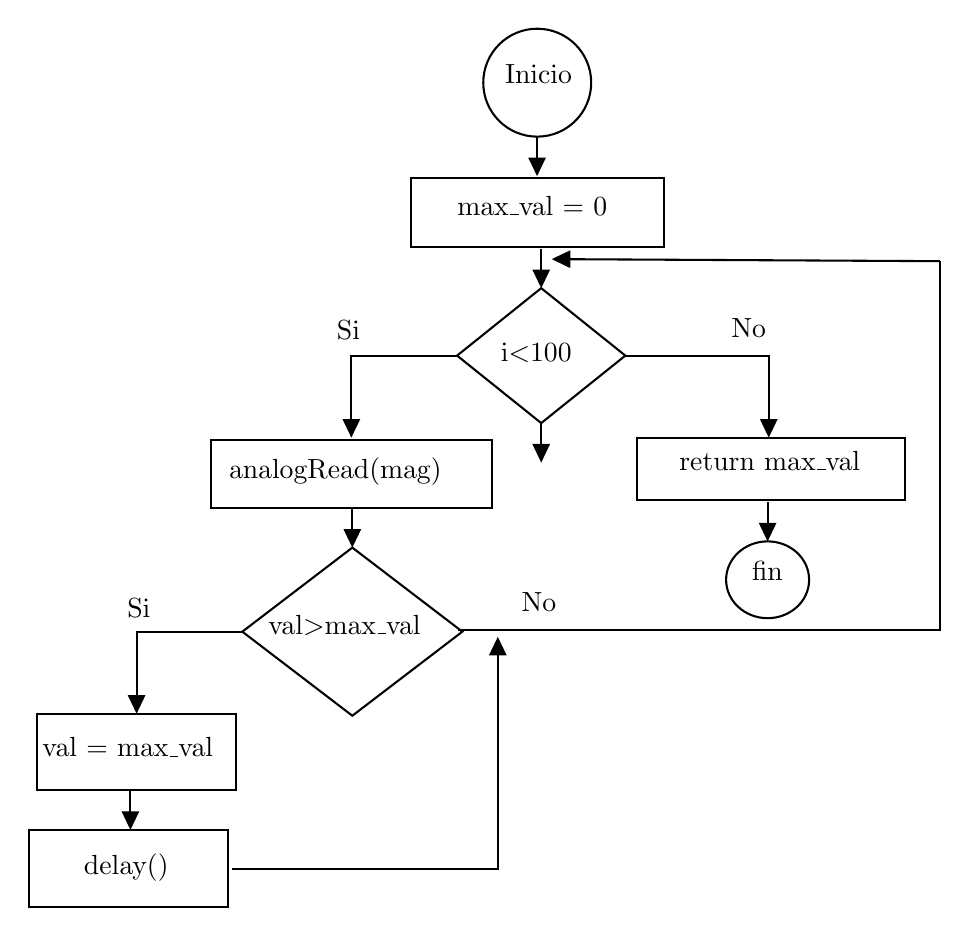
\begin{tikzpicture}[x=0.75pt,y=0.75pt,yscale=-1,xscale=1]
%uncomment if require: \path (0,491); %set diagram left start at 0, and has height of 491

%Flowchart: Connector [id:dp7813495520702245] 
\draw   (320,81) .. controls (320,66.64) and (331.64,55) .. (346,55) .. controls (360.36,55) and (372,66.64) .. (372,81) .. controls (372,95.36) and (360.36,107) .. (346,107) .. controls (331.64,107) and (320,95.36) .. (320,81) -- cycle ;
%Straight Lines [id:da8847526091998554] 
\draw    (345.92,107) -- (345.92,123) ;
\draw [shift={(345.92,126)}, rotate = 270] [fill={rgb, 255:red, 0; green, 0; blue, 0 }  ][line width=0.08]  [draw opacity=0] (8.93,-4.29) -- (0,0) -- (8.93,4.29) -- cycle    ;
%Flowchart: Process [id:dp3892985602062795] 
\draw   (285,127) -- (407,127) -- (407,160) -- (285,160) -- cycle ;
%Flowchart: Decision [id:dp21596588394867888] 
\draw   (347.92,180) -- (388.45,212.5) -- (347.92,245) -- (307.39,212.5) -- cycle ;
%Straight Lines [id:da7204417446380422] 
\draw    (347.92,161) -- (347.92,177) ;
\draw [shift={(347.92,180)}, rotate = 270] [fill={rgb, 255:red, 0; green, 0; blue, 0 }  ][line width=0.08]  [draw opacity=0] (8.93,-4.29) -- (0,0) -- (8.93,4.29) -- cycle    ;
%Straight Lines [id:da451260237829443] 
\draw    (457.55,233) -- (457.55,249) ;
\draw [shift={(457.55,252)}, rotate = 270] [fill={rgb, 255:red, 0; green, 0; blue, 0 }  ][line width=0.08]  [draw opacity=0] (8.93,-4.29) -- (0,0) -- (8.93,4.29) -- cycle    ;
%Straight Lines [id:da49582350632228556] 
\draw    (256.45,233) -- (256.45,249) ;
\draw [shift={(256.45,252)}, rotate = 270] [fill={rgb, 255:red, 0; green, 0; blue, 0 }  ][line width=0.08]  [draw opacity=0] (8.93,-4.29) -- (0,0) -- (8.93,4.29) -- cycle    ;
%Straight Lines [id:da006314317293441896] 
\draw    (327,351) -- (327,367) ;
\draw [shift={(327,348)}, rotate = 90] [fill={rgb, 255:red, 0; green, 0; blue, 0 }  ][line width=0.08]  [draw opacity=0] (8.93,-4.29) -- (0,0) -- (8.93,4.29) -- cycle    ;
%Straight Lines [id:da6050013822698619] 
\draw    (356,166.02) -- (540,167) ;
\draw [shift={(353,166)}, rotate = 0.31] [fill={rgb, 255:red, 0; green, 0; blue, 0 }  ][line width=0.08]  [draw opacity=0] (8.93,-4.29) -- (0,0) -- (8.93,4.29) -- cycle    ;
%Shape: Right Angle [id:dp24954692627046726] 
\draw   (388.45,212.5) -- (457.55,212.5) -- (457.55,233) ;
%Shape: Right Angle [id:dp2914826540765745] 
\draw   (307.39,212.5) -- (256.45,212.5) -- (256.45,233) ;
%Flowchart: Decision [id:dp9064156706798434] 
\draw   (256.92,305) -- (309.92,345.5) -- (256.92,386) -- (203.92,345.5) -- cycle ;
%Straight Lines [id:da6126735924115385] 
\draw    (457,283) -- (457,299) ;
\draw [shift={(457,302)}, rotate = 270] [fill={rgb, 255:red, 0; green, 0; blue, 0 }  ][line width=0.08]  [draw opacity=0] (8.93,-4.29) -- (0,0) -- (8.93,4.29) -- cycle    ;
%Shape: Right Angle [id:dp7943090498770735] 
\draw   (307.98,344.5) -- (540,344.5) -- (540,167) ;
%Straight Lines [id:da7128924347373624] 
\draw    (152.98,366) -- (152.98,382) ;
\draw [shift={(152.98,385)}, rotate = 270] [fill={rgb, 255:red, 0; green, 0; blue, 0 }  ][line width=0.08]  [draw opacity=0] (8.93,-4.29) -- (0,0) -- (8.93,4.29) -- cycle    ;
%Shape: Right Angle [id:dp8866366667209189] 
\draw   (203.92,345.5) -- (152.98,345.5) -- (152.98,366) ;
%Flowchart: Process [id:dp15212318966923655] 
\draw   (105,385) -- (201,385) -- (201,422) -- (105,422) -- cycle ;
%Shape: Right Angle [id:dp9899984887472151] 
\draw   (199,460) -- (327,460) -- (327,367) ;
%Flowchart: Connector [id:dp7268194319410761] 
\draw   (437,320.5) .. controls (437,310.28) and (445.95,302) .. (457,302) .. controls (468.05,302) and (477,310.28) .. (477,320.5) .. controls (477,330.72) and (468.05,339) .. (457,339) .. controls (445.95,339) and (437,330.72) .. (437,320.5) -- cycle ;
%Flowchart: Process [id:dp6713652946060731] 
\draw   (394,252) -- (523,252) -- (523,282) -- (394,282) -- cycle ;
%Straight Lines [id:da15691850789793538] 
\draw    (347.92,245) -- (347.92,261) ;
\draw [shift={(347.92,264)}, rotate = 270] [fill={rgb, 255:red, 0; green, 0; blue, 0 }  ][line width=0.08]  [draw opacity=0] (8.93,-4.29) -- (0,0) -- (8.93,4.29) -- cycle    ;
%Flowchart: Process [id:dp025828036440153967] 
\draw   (189,253) -- (324,253) -- (324,286) -- (189,286) -- cycle ;
%Straight Lines [id:da2671209465635622] 
\draw    (256.92,286) -- (256.92,302) ;
\draw [shift={(256.92,305)}, rotate = 270] [fill={rgb, 255:red, 0; green, 0; blue, 0 }  ][line width=0.08]  [draw opacity=0] (8.93,-4.29) -- (0,0) -- (8.93,4.29) -- cycle    ;
%Straight Lines [id:da2035552754915979] 
\draw    (150,422) -- (150,438) ;
\draw [shift={(150,441)}, rotate = 270] [fill={rgb, 255:red, 0; green, 0; blue, 0 }  ][line width=0.08]  [draw opacity=0] (8.93,-4.29) -- (0,0) -- (8.93,4.29) -- cycle    ;
%Flowchart: Process [id:dp8396019792624998] 
\draw   (101,441) -- (197,441) -- (197,478) -- (101,478) -- cycle ;

% Text Node
\draw (329,71) node [anchor=north west][inner sep=0.75pt]   [align=left] {Inicio};
% Text Node
\draw (306,134) node [anchor=north west][inner sep=0.75pt]   [align=left] {max\_val = 0};
% Text Node
\draw (327,205) node [anchor=north west][inner sep=0.75pt]   [align=left] {i$<$100};
% Text Node
\draw (215,336) node [anchor=north west][inner sep=0.75pt]   [align=left] {val$>$max\_val};
% Text Node
\draw (438,193) node [anchor=north west][inner sep=0.75pt]   [align=left] {No};
% Text Node
\draw (248,194) node [anchor=north west][inner sep=0.75pt]   [align=left] {Si};
% Text Node
\draw (337,325) node [anchor=north west][inner sep=0.75pt]   [align=left] {No};
% Text Node
\draw (147,328) node [anchor=north west][inner sep=0.75pt]   [align=left] {Si};
% Text Node
\draw (106.12,395) node [anchor=north west][inner sep=0.75pt]   [align=left] {val = max\_val};
% Text Node
\draw (413,257) node [anchor=north west][inner sep=0.75pt]   [align=left] {return max\_val};
% Text Node
\draw (196,260) node [anchor=north west][inner sep=0.75pt]   [align=left] {analogRead(mag)};
% Text Node
\draw (126.12,451) node [anchor=north west][inner sep=0.75pt]   [align=left] {delay()};
% Text Node
\draw (448,310) node [anchor=north west][inner sep=0.75pt]   [align=left] {fin};


\end{tikzpicture}
\caption{Diagrama de flujo función mide\_voltaje}
\label{sch3}
\end{figure}